% fig_curves.tex
% Training curves for the path-only configuration (V5 60-epoch run).
% Data points are taken from the validation log every 5 epochs.

\begin{figure}[t]
\centering
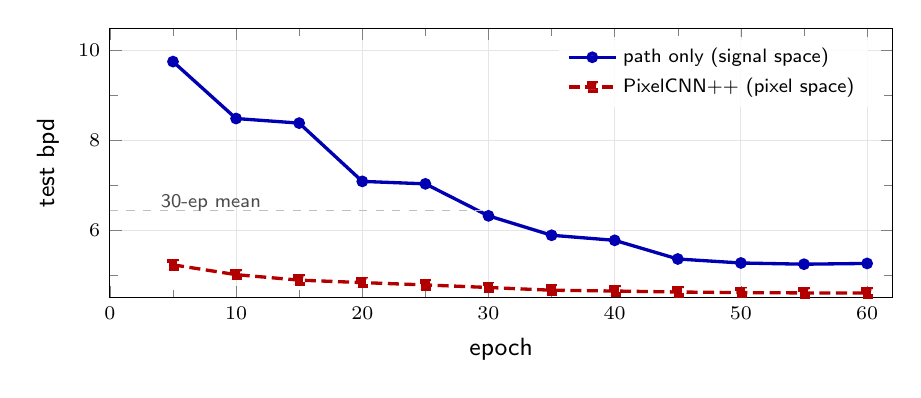
\begin{tikzpicture}
\begin{axis}[
    width=0.95\columnwidth,
    height=5cm,
    xlabel={epoch},
    ylabel={test bpd},
    xmin=0, xmax=62,
    ymin=4.5, ymax=10.5,
    grid=major,
    grid style={gray!20},
    minor tick num=1,
    legend pos=north east,
    legend cell align={left},
    legend style={font=\sffamily\scriptsize, draw=none, fill=white,
                  fill opacity=0.85, text opacity=1},
    label style={font=\sffamily\small},
    tick label style={font=\sffamily\scriptsize},
    every axis plot/.append style={very thick},
]
% V5 path-only (signal-space) -- from 60-epoch run
\addplot[color=blue!70!black, mark=*, mark size=1.5pt] coordinates {
  (5, 9.756) (10, 8.487) (15, 8.385) (20, 7.086) (25, 7.031)
  (30, 6.318) (35, 5.885) (40, 5.772) (45, 5.356) (50, 5.267)
  (55, 5.240) (60, 5.257)
};
\addlegendentry{path only (signal space)}

% PixelCNN++ -- from 60-epoch run
\addplot[color=red!70!black, mark=square*, mark size=1.5pt,
         dash pattern=on 4pt off 2pt] coordinates {
  (5, 5.226) (10, 5.007) (15, 4.885) (20, 4.830) (25, 4.778)
  (30, 4.721) (35, 4.660) (40, 4.642) (45, 4.620) (50, 4.607)
  (55, 4.600) (60, 4.598)
};
\addlegendentry{PixelCNN++ (pixel space)}

% Reference line for V5 30-epoch path-only
\draw[gray!50, dashed] (axis cs:0,6.432) -- (axis cs:30,6.432);
\node[font=\sffamily\scriptsize, gray!60!black] at (axis cs:8,6.6)
    {30-ep mean};

\end{axis}
\end{tikzpicture}
\caption{Validation bits-per-pixel during training. Signal-space
(blue) is the path-only configuration of \cref{ssec:main}; pixel-space
(red, dashed) is the matched-parameter PixelCNN++ baseline of
\cref{ssec:pixelcnn}. Both are single-seed runs over 60 epochs. The
dashed grey line marks the multi-seed mean of the path-only
configuration at 30 epochs ($\SI{6.43}{}$ bpd).}
\label{fig:curves}
\end{figure}
